\input preamble.tex
\noindent
\section*{Industrielektronikk Øving 03 - Seriekobling av to motstandere}

I denne øvingen skal du bruke koblingsbrettet til å koble to motstandere i serie. 

\noindent \begin{center}
\begin{figure}[H]
\noindent \begin{centering}
%\includegraphics[angle=90,width=16cm]{\string"tegninger/Elektroteknikk - Breadboard\string".pdf}\vspace{2cm}
\par\end{centering}
\noindent \begin{centering}
%\includegraphics[width=16cm]{\string"tegninger/Elektroteknikk - koblingsbrett\string".jpg}
\par\end{centering}
$$\includegraphics[width=10cm]{./lIndustrielektronikk03.eps}$$
\end{figure}
\par\end{center}

\subsubsection*{Utstyr du trenger}
\begin{itemize}
\item Labbrettet
\item Motstand med en verdi på 2700$\Omega$ (2k7) $R_1$
\item Motstand med en verdi på 2200$\Omega$ (2k2) $R_2$
\item Multimeter
\end{itemize}

\subsubsection*{Oppgaven}

Koble de to motstandene i serie ved hjelp av koblingsbrettet. Lag et skjema over den samme kretsen. 
\begin{enumerate}
	
		\item Regn ut spenningen over Hver av motstandene ($R_1$ og $R_2$)
		\item Mål spenningen over hver av motstandene($R_1$ og $R_2$)
		\item Regn ut strømmen i kretsen
		\item Koble et ampermeter i kretsen. Hva blir strømmen.
		\item Regn ut total resistanden i kretsen 
		\item Koble om slik at motstandene er i serie men ikke tilkoblet spenningskilden og mål total resistansen
\end{enumerate}

\subsubsection*{Innlevering}

Skriv en labrapport og lever på OneNote\\
\underbar{file ./lIndustrielektronikk03.tex}
\vskip 5pt 

\end{document}

